\chapter{Integration Tests}

\section{CDU and Sensor}
\subsection{Integration test case 1: Sensor getinfo request}
\textbf{Purpose:}\\
The purpose of the test\\

\textbf{Test equipment:}
\begin{itemize}
\item Analog Discovery USB oscilloscope
\item MPLAB X IDE
\item Explorer 16 board
\item ICD 3 Debugger
\item CDU stub
\item Sensor node with address 1
\end{itemize}

\textbf{Procedure:}\\
Apply 20 V on the P+ and P- pins of the CDU. Connect a sensor node to B+ and B- pins of the CDU. Connect the Explorer 16 board to the CDU circuit. Using the ICD 3 debugger, send a full message containing start sequence, address: "1" and function code: "1". Record what have been received on the sensor node circuit.\\

\textbf{Expected Result:}\\
A full message with address: "1" and function code: "1" has been received on the sensor node circuit.\\

\textbf{Actual Result:}\\
\begin{table}[H]
\centering
\begin{tabular}{|p{2cm}|p{2cm}|p{3cm}|p{2cm}|}\hline
\textbf{Test case:} & \textbf{Date:} & \textbf{Measurement:} & \textbf{Result:} \\ \hline
1 & - & - & - \\ \hline
\end{tabular}
\end{table}

\begin{figure}[H]
\centering
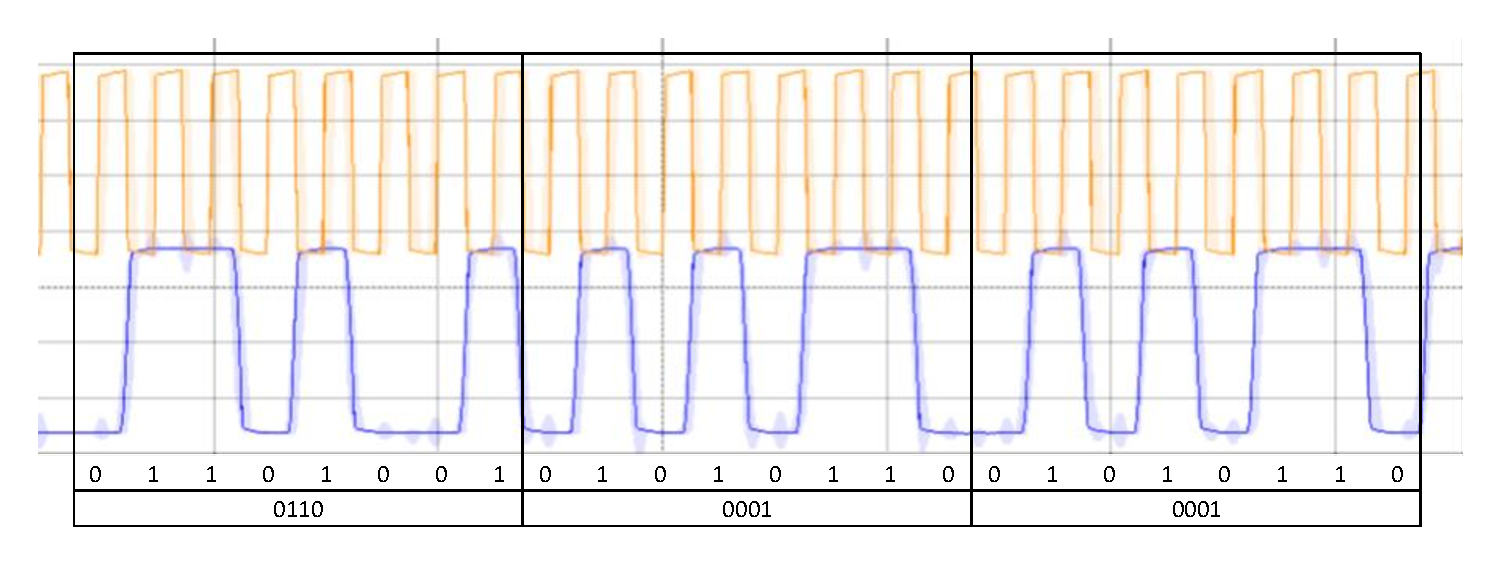
\includegraphics[width=0.8\textwidth]{billeder/CDUtestcase9}
\caption{Test Case 1 Result}
\label{fig:InteTestCase1}
\end{figure}

\textbf{Comment and remarks:}\\
-\\

\subsection{Integration test case 2: Sensor getdata request}
\textbf{Purpose:}\\
The purpose of the test\\

\textbf{Test equipment:}
\begin{itemize}
\item Analog Discovery USB oscilloscope
\item MPLAB X IDE
\item Explorer 16 board
\item ICD 3 Debugger
\item CDU stub
\item Sensor node with address 1
\end{itemize}

\textbf{Procedure:}\\
Apply 20 V on the P+ and P- pins of the CDU. Connect a sensor node to B+ and B- pins of the CDU. Connect the Explorer 16 board to the CDU circuit. Using the ICD 3 debugger, send a full message containing start sequence, address: "1" and function code: "2". Record what have been received on the sensor node circuit.\\

\textbf{Expected Result:}\\
A full message with address: "1" and function code: "2" has been received on the sensor node circuit.\\

\textbf{Actual Result:}\\
\begin{table}[H]
\centering
\begin{tabular}{|p{2cm}|p{2cm}|p{3cm}|p{2cm}|}\hline
\textbf{Test case:} & \textbf{Date:} & \textbf{Measurement:} & \textbf{Result:} \\ \hline
2 & - & - & - \\ \hline
\end{tabular}
\end{table}


\textbf{Comment and remarks:}\\
-\\

\subsection{Integration test case 3: Sensor respond to getinfo}
\textbf{Purpose:}\\
The purpose of the test\\

\textbf{Test equipment:}
\begin{itemize}
\item Analog Discovery USB oscilloscope
\item MPLAB X IDE
\item Explorer 16 board
\item ICD 3 Debugger
\item CDU stub
\item Sensor node with address 1
\end{itemize}

\textbf{Procedure:}\\
hest

\textbf{Expected Result:}\\
hest

\textbf{Actual Result:}\\
\begin{table}[H]
\centering
\begin{tabular}{|p{2cm}|p{2cm}|p{3cm}|p{2cm}|}\hline
\textbf{Test case:} & \textbf{Date:} & \textbf{Measurement:} & \textbf{Result:} \\ \hline
3 & - & - & - \\ \hline
\end{tabular}
\end{table}


\textbf{Comment and remarks:}\\
-\\

\subsection{Integration test case 4: Sensor respond to getdata}
\textbf{Purpose:}\\
The purpose of the test\\

\textbf{Test equipment:}
\begin{itemize}
\item Analog Discovery USB oscilloscope
\item MPLAB X IDE
\item Explorer 16 board
\item ICD 3 Debugger
\item CDU stub
\item Sensor node with address 1
\end{itemize}

\textbf{Procedure:}\\
hest

\textbf{Expected Result:}\\
hest

\textbf{Actual Result:}\\
\begin{table}[H]
\centering
\begin{tabular}{|p{2cm}|p{2cm}|p{3cm}|p{2cm}|}\hline
\textbf{Test case:} & \textbf{Date:} & \textbf{Measurement:} & \textbf{Result:} \\ \hline
4 & - & - & - \\ \hline
\end{tabular}
\end{table}


\textbf{Comment and remarks:}\\
-\\

\subsection{Integration test case 5: Sensor unknown request}
\textbf{Purpose:}\\
The purpose of the test\\

\textbf{Test equipment:}
\begin{itemize}
\item Analog Discovery USB oscilloscope
\item MPLAB X IDE
\item Explorer 16 board
\item ICD 3 Debugger
\item CDU stub
\item Sensor node with address 1
\end{itemize}

\textbf{Procedure:}\\
hest

\textbf{Expected Result:}\\
hest

\textbf{Actual Result:}\\
\begin{table}[H]
\centering
\begin{tabular}{|p{2cm}|p{2cm}|p{3cm}|p{2cm}|}\hline
\textbf{Test case:} & \textbf{Date:} & \textbf{Measurement:} & \textbf{Result:} \\ \hline
5 & - & - & - \\ \hline
\end{tabular}
\end{table}


\textbf{Comment and remarks:}\\
-\\


\section{CDU and PC}
\subsection{Integration test case 6: PC sends getdata request to CDU}
\textbf{Purpose:}\\
The purpose of the test\\

\textbf{Test equipment:}
\begin{itemize}
\item Analog Discovery USB oscilloscope
\item MPLAB X IDE
\item Explorer 16 board
\item ICD 3 Debugger
\item CDU stub
\item Sensor node with address 1
\end{itemize}

\textbf{Procedure:}\\
hest

\textbf{Expected Result:}\\
hest

\textbf{Actual Result:}\\
\begin{table}[H]
\centering
\begin{tabular}{|p{2cm}|p{2cm}|p{3cm}|p{2cm}|}\hline
\textbf{Test case:} & \textbf{Date:} & \textbf{Measurement:} & \textbf{Result:} \\ \hline
6 & - & - & - \\ \hline
\end{tabular}
\end{table}


\textbf{Comment and remarks:}\\
-\\

\subsection{Integration test case 7: PC sends unknown request to CDU}
\textbf{Purpose:}\\
The purpose of the test\\

\textbf{Test equipment:}
\begin{itemize}
\item Analog Discovery USB oscilloscope
\item MPLAB X IDE
\item Explorer 16 board
\item ICD 3 Debugger
\item CDU stub
\item Sensor node with address 1
\end{itemize}

\textbf{Procedure:}\\
hest

\textbf{Expected Result:}\\
hest

\textbf{Actual Result:}\\
\begin{table}[H]
\centering
\begin{tabular}{|p{2cm}|p{2cm}|p{3cm}|p{2cm}|}\hline
\textbf{Test case:} & \textbf{Date:} & \textbf{Measurement:} & \textbf{Result:} \\ \hline
7 & - & - & - \\ \hline
\end{tabular}
\end{table}


\textbf{Comment and remarks:}\\
-\\